\begin{figure*}[t]
\centering
\vspace{2pt}
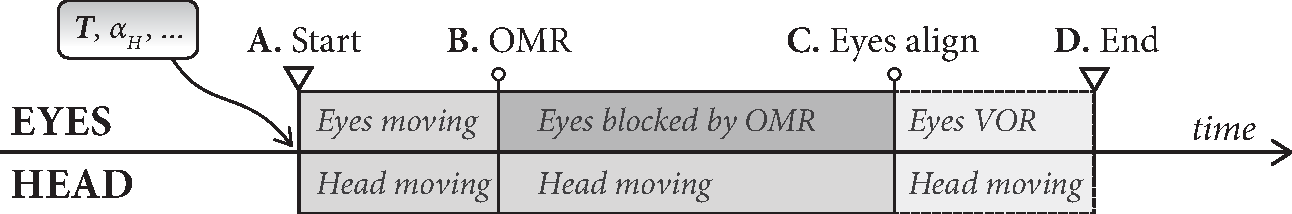
\includegraphics[width=0.8\textwidth]{Figures/AndristGazeModel.pdf}
\caption{Gaze shift phases in the baseline gaze model.}
\vspace{-10pt}
\label{fig:AndristGazeModel}
\end{figure*}

The visual artifacts described in the previous section occur because human gaze mechanics do not necessarily apply to non-human characters. To create a model that can be applied more broadly, we extend an existing model of human gaze, under the premise that we want to retain as much of the human behavior as possible. In this work, we build on the model for gaze shifts proposed by Andrist et al. \cite{andrist2012headeye}, which we hereafter refer to as the \textit{baseline} gaze model, as a state-of-the-art model of gaze that has been validated in previous studies \cite{andrist2012headeye,andrist2012designing} and shown to achieve significant communicative effects.

\subsection{Baseline Model}
\label{sec:baseline}
Figure~\ref{fig:AndristGazeModel} provides an overview of gaze shifts generated by the baseline model. Before the gaze shift begins, the model is provided with a set of parameters, including gaze target position $T$ and head alignment $\alpha_H$. Head alignment specifies how much the head should align with the gaze target; it ranges from 0 (using minimal head motion) to 1 (fully align the head with the target). At the start of the gaze shift (A), eyes and head begin rotating toward the target together. Since eyes move much faster than the head does, they quickly get ahead and reach their OMR (B), where they remain blocked as the head catches up. Eventually the head rotates far enough to bring the eyes into alignment with the target (C). VOR locks the eyes onto the target as the head catches up. Depending on the specified head alignment, the head will either stop moving immediately or continue rotating until it reaches the required alignment with the target (D). For further details of the model, please see \cite{andrist2012headeye}.

When the eyes are moving freely (phase A to B), their motion is governed by the velocity profile shown in Figure~\ref{fig:VelocityProfile}. A very similar profile is also used for head motion. Peak velocity $V_{MAX}$ in the profile is not constant and is instead computed at the start of every gaze shift based on the magnitude of the upcoming eye movement, according to the following formula:
\begin{eqnarray} \label{eq:AndristVmax}
V_{MAX} &=& (\frac{2}{75} A_{MIN} + \frac{1}{6})V_0 \\
A_{MIN} &=& min( \mathop{min}_{j \in Eyes}(D_j), OMR ) \nonumber
\end{eqnarray}
where $D_j$ is rotational distance (in degrees) that the eye $j$ has to rotate before reaching the target. $V_0$ is a user-specifiable velocity parameter, normally left at the default value of $150 deg/s$.

The gaze model also features a model of eye blinks that probabilistically generates idle blinks at a constant average rate and gaze-evoked blinks that occur during the gaze shift based on the model originally described in \cite{peters2010animating}. Evinger et al. \cite{evinger1994lookleap} hypothesize the purpose of gaze-evoked eye blinks is to protect the eye during the movement and lubricate the cornea.

\begin{figure}[!b]
\centering
\vspace{-6pt}
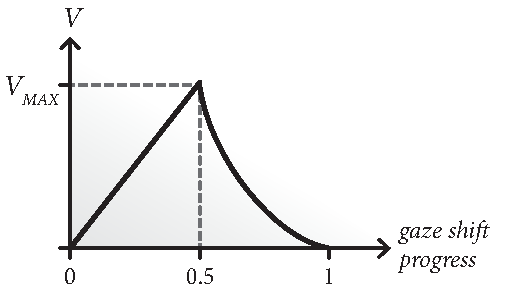
\includegraphics[width=0.40\textwidth]{Figures/VelocityProfile.pdf}
\caption{Velocity profile governing eye movements. Eyes accelerate until they reach peak velocity $v_{MAX}$ halfway through the gaze shift and then decelerate until the end of the gaze shift.}
\vspace{-10pt}
\label{fig:VelocityProfile}
\end{figure}

\subsection{Gaze Shifts for Stylized Characters}

In consideration of the challenges associated with applying a model of human gaze behavior to stylized or non-human characters, we extend the model above with parameters that account for the non-realistic anatomy of the latter and techniques to explicitly avoid the artifacts described in the previous section, while seeking to maintain as much of the human movement as possible.
Our extensions fall into three categories.
First, we introduce changes to how the target pose of the eyes and head is computed in order to prevent the occurrence of anomalous poses. Second, we extend the computation of eye movement dynamics to account for variable physical constraints of the exaggerated geometries that are common in stylized characters. Third, we manipulate the timings of gaze-evoked eye blinks to co-occur with potential visual artifacts to conceal them.

To specify the character's specific properties, we introduce four designer-adjustable parameters to the model. Eye width, $W$, is the width of the eye as a factor of the width of the typical human eye (approximately $2.5 cm$), ranging from 1 to 3 in the characters we encountered. Eye strength $F$ allows for tuning the strength of the character's eye muscles relative to that of a human. Additionally, we replace the single parameter of the $OMR$ in humans with parameters $OMR_{IN}$ and $OMR_{OUT}$ that afford asymmetric eye motion by specifying the inward and outward OMR limits (in angle degrees), respectively. Eye width, $W$, and OMR parameters, $OMR_{IN}$ and $OMR_{OUT}$, can be determined from face geometry, while we use the value of $W^3/3$ for eye strength, $F$, which works well across a range of characters.
% NOTE: Extended discussion of new model parameters with instructions on how to tune them. -- Tomislav

\begin{figure}[b]
\centering
\vspace{-6pt}
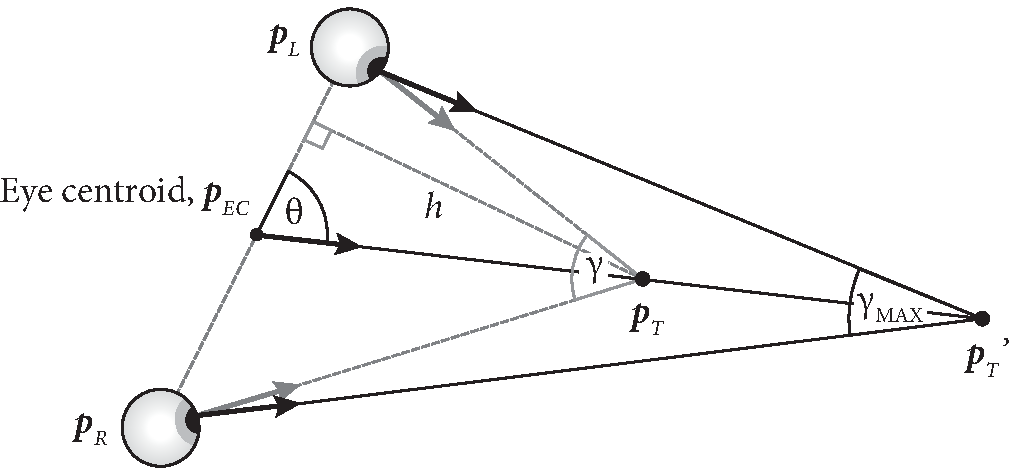
\includegraphics[width=0.48\textwidth]{Figures/CrosseyednessRemoval.pdf}
\caption{Our approach to reducing cross-eyedness in the target gaze pose.}
\vspace{-6pt}
\label{fig:CrosseyednessRemoval}
\end{figure}

\begin{figure}[t]
\centering
\vspace{2pt}
\includegraphics[width=0.48\textwidth]{Figures/CrosseyednessFixExample-small.pdf}
\caption{Cross-eyedness and its reduction. Left: Cross-eyed character. Right: Cross-eyedness reduced by our model.}
\vspace{-12pt}
\label{fig:CrosseyednessFixExample}
\end{figure}

\begin{figure}[!b]
\centering
\vspace{-6pt}
\includegraphics[width=0.48\textwidth]{Figures/EyeDivergenceFixExample-small.pdf}
\caption{Example of eye divergence handling. Top: VOR begins to move the left eye immediately on alignment. Bottom: Our model ensures that VOR begins eye movement only after the right eye has aligned.}
\vspace{-6pt}
\label{fig:EyeDivergenceFixExample}
\end{figure}

\subsubsection{Target Pose Adaptation}
\label{sec:TargetPoseAdaptation}

The baseline model, when applied to a stylized character with large eyes, is prone to bring the eyes into a noticeably cross-eyed state. If the character's eyes are asymmetric, then the eyes can also be led into a divergent state, which will become noticeable as the leading eye reaches the gaze target and VOR reverses its direction of movement. To avoid these artifacts, our model adapts the target pose of the eyes and head at the beginning of the gaze shift by adjusting effective gaze target position and OMR parameters.

\textit{Cross-eyedness Removal} -- Our approach to remove cross-eyedness is illustrated in Figure~\ref{fig:CrosseyednessRemoval}. We measure cross-eyedness as the angle between the gaze directions of the two eyes, $\gamma$. Allowable cross-eyedness is defined by a threshold $\gamma_{MAX}$, which we leave at a default value of $0.002^{\circ}$ for the examples in this paper.
% NOTE: Made it more clear that the parameter should be left as is unless there is a good reason to tweak it. -- Tomislav
We define the \textit{effective target position} as the position behind the physical gaze target that the eyes can converge on without violating the cross-eyedness threshold. It is calculated by moving the target position away from the character to reduce $\gamma$ below the threshold value $\gamma_{MAX}$,
\begin{eqnarray}
T' = E + \frac{T-E}{||T-E||} \frac{ \sin( \theta + \gamma_{MAX}/2 ) }{ sin( \gamma_{MAX}/2 ) } ||L-E||.
\end{eqnarray}
The above technique is effective at reducing cross-eyedness as shown in Figure~\ref{fig:CrosseyednessFixExample}.

The cross-eyedness removal technique is applied in a view-dependent manner; we may only apply it if the viewer cannot notice it from the current viewpoint.

If the viewer is the gaze target, they may notice the character is looking a bit ``past'' them if cross-eyedness removal is applied.
Therefore, the cross-eyedness threshold $\gamma_{MAX}$ is adjusted based on the target viewing angle $\phi_T$, which we define as the angle between the viewer's gaze direction and the character's gaze direction at the target pose. $\gamma_{MAX}$ is adjusted as follows:
\begin{eqnarray}
\gamma\,'_{MAX} &=& 2OMR_{IN} + ( \gamma_{MAX} - 2OMR_{IN} ) p_{\phi} \\
p_{\phi} &=& \phi_T / ( 9.6W ),~ 0 \le t \le 1 \nonumber
\end{eqnarray}
where $OMR_{IN}$ is inward OMR of the eye, and $W$ is the eye width parameter. The $9.6^{\circ}$ constant is derived from parameters of the viewing cone in which humans are able to detect subtle differences in gaze direction \cite{argyle1976gaze}. We scale this value by $W$, as larger eyes may make such judgements easier. The viewing cone parameter, $p_{\phi}$, expresses the drop-off in judgement accuracy from the center of the cone towards the edge. We use $p_{\phi}$ to vary allowable cross-eyedness from the mechanical limit, $2OMR_{IN}$, at the center to $\gamma_{MAX}$ at the cone's edge and beyond.

\begin{figure*}[t]
\centering
\includegraphics[width=0.98\textwidth]{Figures/GazeDynamicsExample1-small.pdf}
\caption{Gaze shifts with different gaze dynamics. Top: Baseline model. The gaze shift contains the artifacts stuck eye, OMR-block, and eye retraction. Bottom: Our model. The artifacts of the baseline model are reduced.}
\vspace{-10pt}
\label{fig:GazeDynamicsExample}
\end{figure*}

\textit{Eye Divergence} -- A consequence of OMR asymmetry, eye divergence is handled by allowing the eyes to diverge during the gaze shift and imposing the principle that VOR for both eyes must trigger \emph{at the same time}. The leading eye will always overshoot the gaze target by a small amount and only begin moving in the opposite direction (due to VOR) when the trailing eye has reached the target. This behavior prevents the leading eye from aligning exactly with the target, as the accumulated overshoot rotation introduces an offset into the eye's target rotation. However, much like with cross-eyedness removal, this minor deviation from correct gaze convergence is difficult to detect. This technique is therefore an effective way of eliminating disconjugate eye movements as shown in Figure~\ref{fig:EyeDivergenceFixExample}.

As with cross-eyedness removal, eye divergence is applied in a view-dependent manner. The target overshoot introduced by the technique may be noticeable to the viewer at very low viewing angles, which we therefore adjust using the viewing cone parameter, $p_{\phi}$, that we defined in the previous subsection. Specifically, we scale the outward OMR based on target viewing angle, $\phi_T$,

\begin{equation}
OMR_{OUT}' = OMR_{IN} + ( OMR_{OUT} - OMR_{IN} ) p_{\phi}
\end{equation}

This adjustment ensures that outward OMR will contract at low $\phi_T$, making the OMR symmetrical.

\subsubsection{Gaze Dynamics}

Because most stylized characters do not have the same proportions and oculomotor constraints as humans, our model includes specific extensions to the baseline model to consider the additional character parameters described above to compute its dynamics. To preserve the characteristics of the movement, the model uses the velocity profile in Figure~\ref{fig:VelocityProfile} but changes the manner in which $V_{MAX}$ is computed by defining peak velocities, $V_{MAX,j}$, for each eye, departing from the assumption that both eyes have the same peak velocity. It uses eye width, $W$, and muscle strength, $F$, to compute these velocities. As volume---and therefore mass---increases with $W^3$, peak velocity is scaled down by the same factor. $F$ is used to compute an intermediate parameter $F'$, which varies depending on how much the head contributes to the gaze shift. We compute $F'$ as follows:

\begin{equation}
F' = ( 1 - \alpha_H ) W^3 + \alpha_H F.
\end{equation}

The parameter $\alpha_H$ specifies how much the head contributes to the gaze shift. When the head carries the eyes through most of the gaze shift (high $\alpha_H$), eye velocity should be lower in order to prevent the eyes from appearing improbably fast. When the head moves only a small distance, the eyes should move more quickly to prevent the gaze shift from appearing slow and sluggish.

Our method must also account for OMR asymmetry to prevent artifacts such as \textit{stuck eye} from occurring. Assume that $D_{OMR,j}$ is the distance that eye $j$ can rotate before reaching OMR, while $A_{MAX}$ is the highest rotational distance to OMR for each eye. The peak velocity is scaled by $D_{OMR,j}/A_{MAX}$ to slow down the eye that has less rotation to complete, thus ensuring that both eyes reach OMR at the same time.

Finally, we introduce a velocity multiplier parameter, $\chi$, and apply it uniformly to eye and head velocities in order to make the character's gaze appear livelier or more expressive and to better reflect their personality and mood. By default, $\chi$ is set to $1$, although we use values between $1.2$ and $1.7$ for our stylized characters.
% NOTE: Clarified how the parameter might be used by explaining how we use it. -- Tomislav

We introduce these modifications to Equation~\ref{eq:AndristVmax} to create the following updated equation for calculating peak velocity:

\begin{equation}
V_{MAX,j} = \frac{F}{W^3}( \frac{2}{75} A_{MAX} + \frac{1}{6} ) \frac{D_{OMR}}{A_{MAX}} \chi V_0 %+ 3 \delta V_{MAX,H}
\end{equation}

The first, third, and fourth terms implement our modifications to gaze dynamics. The second term speeds up or slows down the eyes depending on eye movement distance and is similar to the term used by the baseline model to calculate peak velocity, except that $A_{MIN}$ is replaced by $A_{MAX}$.

%The rightmost term $3 \delta v_{MAX,H}$ addresses an issue with the original gaze model. For certain rare gaze shifts, the angle $\delta$ between eye and head rotation directions may become much greater than 0; eyes could even end up moving in the opposite direction of the head. In these cases, the head is slowing down the eyes rather than helping them reach the target, so the above term speeds up the eyes to compensate for the opposing head rotation.
% Since this is a bugfix of the original model, maybe it doesn't need to be here? It muddles the story somewhat, and takes up space...

Using the above method of calculating peak velocity reduces artifacts related to gaze dynamics, producing gaze shifts that appear smoother and more lifelike. The stuck eye artifact is largely eliminated; the amount of time spent in the state of OMR-block is greatly reduced; and VOR causes less eye retraction (Figure~\ref{fig:GazeDynamicsExample}). The eye retraction cannot be completely eliminated, as some VOR must occur to achieve the specified head alignment and thus produce desired communicative effects.

\begin{figure}[!b]
\centering
\vspace{-2pt}
\includegraphics[width=0.48\textwidth]{Figures/GazeEvokedBlinkVOR-small.pdf}
\caption{A gaze-evoked eye blink during the VOR phase. The blink conceals the retraction in the left eye.}
\vspace{-6pt}
\label{fig:GazeEvokedBlinkVOR}
\end{figure}

\subsubsection{Gaze-evoked Eye Blinks}

As described in section~\ref{sec:baseline}, the baseline gaze model also incorporates an ancillary model of gaze-evoked eye blinks. The model probabilistically determines whether or not a gaze-evoked eye blink will occur at the beginning of the gaze shift.
%However, the timing of the blink is deterministic---if generated, the blink occurs immediately at the start of the gaze shift. However,
In humans, eye blinks can occur at any point during the gaze shift. Our model uses this flexibility to time gaze-evoked eye blinks to co-occur with potential eye retraction artifacts to conceal them (Figure~\ref{fig:GazeEvokedBlinkVOR}).

\begin{figure}[!b]
\centering
\vspace{-6pt}
\includegraphics[width=0.48\textwidth]{Figures/PerformativeGazeExample-small.pdf}
\caption{A performative gaze shift. Top: The character fully aligns with the red sphere. Bottom: The character partially aligns with the target ($\alpha_E = 0.7$) but still appears to be gazing at it, because it has achieved screen-space alignment.}
\vspace{-6pt}
\label{fig:PerformativeGazeExample}
\end{figure}

\begin{figure}[t]
\centering
\vspace{2pt}
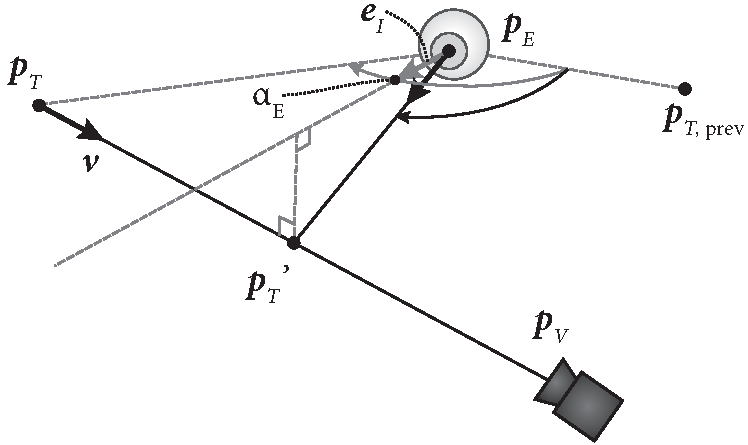
\includegraphics[width=0.5\textwidth]{Figures/EyeAlignment.pdf}
\caption{The calculation of the effective gaze target position in a performative gaze shift.}
\vspace{-10pt}
\label{fig:EyeAlignment}
\end{figure}

Our implementation generates a gaze-evoked eye blink at the start of the gaze shift, using the same probabilistic method as in the baseline model. However, when determining the timing of the blink, it considers estimates of the duration of the VOR phase of the gaze shift, $T_{VOR}$, and the time when VOR phase will begin, $t_{VOR}$. If $T_{VOR}$ is greater than a threshold value, then the gaze-evoked blink is scheduled to begin at $t_{VOR} - 0.35T_{B}$, where $T_B$ is a probabilistically generated blink duration, and $0.35T_B$ is the time when eyes are fully closed.

\subsection{Performative Gaze Shifts}

While humans use gaze primarily to direct their attention to or seek information from their environment, in acting and cartoon animation, these primary goals are replaced by communicating ideas to and creating engagement with an audience. These goals are achieved by performing partial gaze shifts in the general direction of the object of interest and/or attention in order to convey the idea that the character is looking at the object without precisely aligning gaze with it. This performative behavior allows the character to retain partial alignment with the audience, which recent research has shown to improve how the viewer evaluates the character in measures such as engagement, likability, and trustworthiness \cite{andrist2012designing}.

Our model provides explicit support for partial gaze shifts by exposing the eye alignment parameter, $\alpha_E$, which allows the designer to specify the desired amount of alignment with the target. An $\alpha_E$ of $1$ causes the eyes to fully align with the target in a way that is similar to human gaze. We find that values between $0.6$ and $1$ produce good performative effects.
% NOTE: More detailed explanation of how the parameter can be tweaked -- Tomislav
With parameter values smaller than $1$, the character will gaze toward a point directly between the gaze target and the viewer, which we call the \textit{effective gaze target}. In order to convince the viewer that the character is gazing toward the real target, the two targets must occupy the same screen-space position, as illustrated in Figure~\ref{fig:PerformativeGazeExample}.

Figure~\ref{fig:EyeAlignment} illustrates how correct partial eye alignment is achieved. We compute the intermediate rotation of each eye, $E$, using $q_I = slerp ( q_S, q_T, \alpha_E )$, where $q_S$ and $q_T$ are eye rotations in the source and target pose, respectively. At this rotation, gaze direction is given by vector $\mathbf{e_I}$. The view direction, $\mathbf{v}$, points from the target $T$ to the viewer. Effective gaze target position, $\mathbf{T'}$, is the point on $\mathbf{v}$ that is closest to $\mathbf{e_I}$.

Similar to the target pose adaptation techniques described in Section~\ref{sec:TargetPoseAdaptation}, eye alignment is applied in a view-dependent manner. With low target viewing angles, $\phi_T$, the model enforces eye alignment to prevent the viewer from noticing that the character is not actually gazing at them by automatically adjusting it using the viewing cone parameter, $p_{\phi}$, as follows:

\begin{equation}
\alpha_E' = 1 - p_{\phi} + \alpha_E p_{\phi}.
\end{equation}

\begin{figure*}[t]
\centering
\includegraphics[width=1\textwidth]{Figures/TestCases-small.pdf}
\caption{The characters used in our evaluation. From left to right: RealisticFemale1, RealisticFemale2, SemiStylizedFemale, StylizedFemale, StylizedMale, EmotiGuy, Jack, Donkey, Fish, and NastyMonster.}
\vspace{-10pt}
\label{fig:TestCases}
\end{figure*}